\documentclass{article}



\usepackage{graphicx}%allows import messages
\usepackage{float}%allow control float position
\usepackage{hyperref}
\hypersetup{ % link to the references e.g. the sections
    colorlinks,
    citecolor=black,
    filecolor=black,
    linkcolor=black,
    urlcolor=black }
%-------------------------------------------------------------------------------------------------------------

\begin{document}
\begin{titlepage}
		\begin{center}% puts the text on the right side of the page
		{\huge{protocol}}\\ % \\ makes a new line
		[2cm]
		{\large Crownstone B.V }\\
		[15cm]
		\end{center} 
		\begin{flushright}
		{\large Ilhan Delic \\}
		\# 0914619 \\
		november 2019 \\
		\end{flushright}	
\end{titlepage}
% here you can place a summary 
% \section*{Summary}
%text \cleardoublepage 
%-------------------------------------------------------------------------------------------------------------
%table of contents 
\tableofcontents
\thispagestyle{empty}
\cleardoublepage %clears the rest of the page
%-------------------------------------------------------------------------------------------------------------
\pagenumbering{arabic}%the western number system
\section{introduction}\label{sec:intro}% reference
This is the documentation for the protocol for the hub. I'll describe my thinking and design process for this protocol 
%-------------------------------------------------------------------------------------------------------------
\section{Design}\label{sec:design}

In order to get a better idea of how to set up a protocol i had to make a design of how the communication will flow between the parts. In order to get the data that's stored on the cloud and show it to the hub you could make an event server which uses SSE to show the current dynamic data. The communication needs to start at the hub side and the hub needs to make a REST call to the cloud in order to start things off. when that has been done the next step would be for the event server to push the data that is requested from the hub. With this way you get the data immediately.\\

\label{fig:protocolDraft}	
	\begin{figure}[H]
	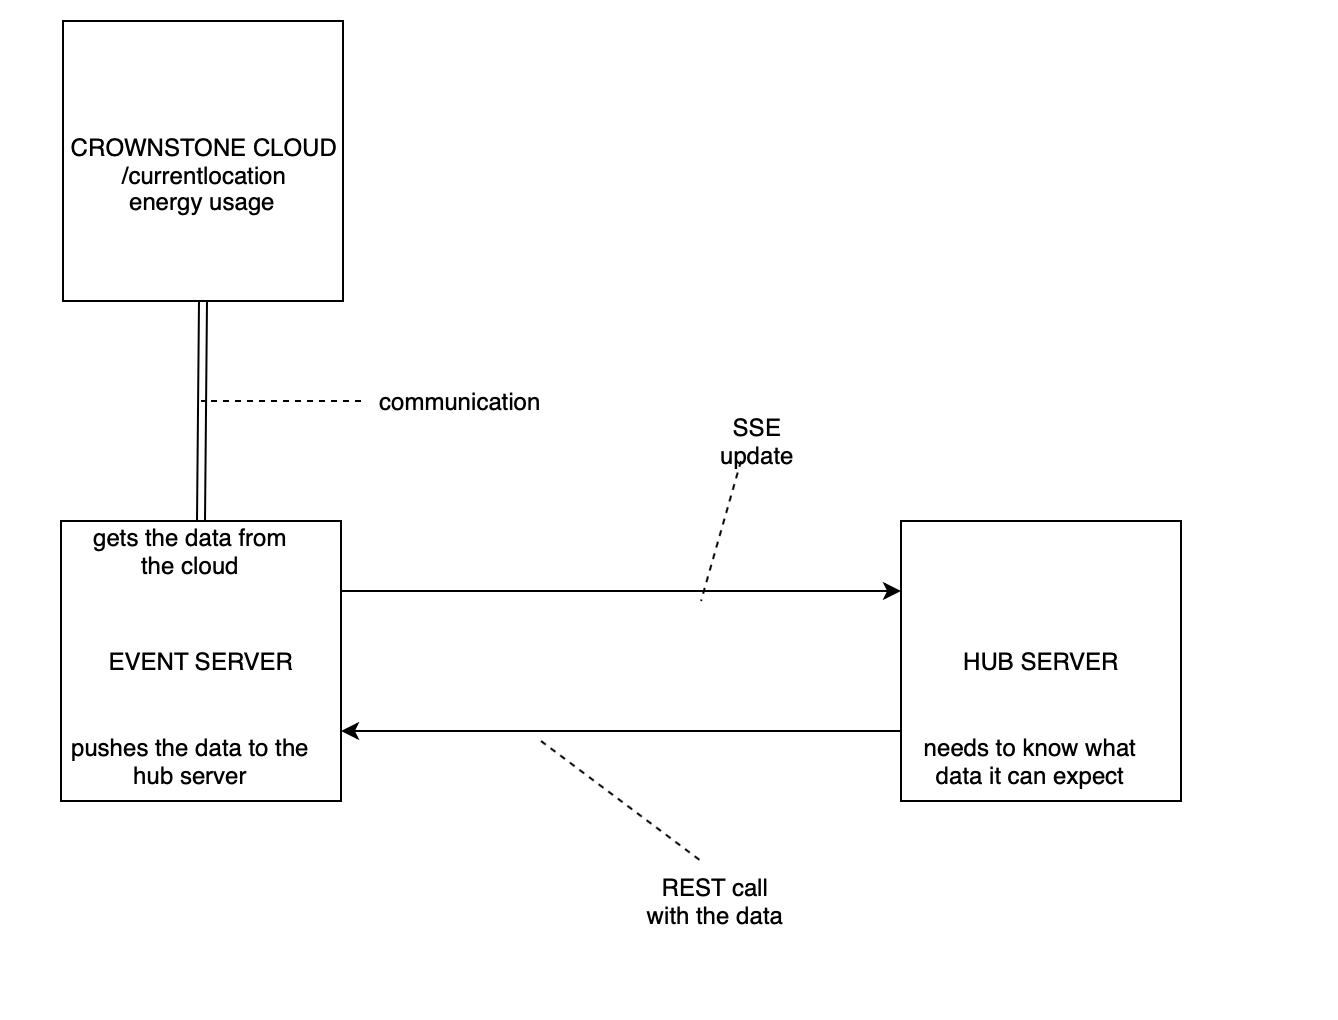
\includegraphics[width=5in]{pictures/protocolDraft.png}
	\caption[Optional caption]{protocol draft design}
	\end{figure}
	

\section{functionality}



%-------------------------------------------------------------------------------------------------------------
\end{document}